% slc-screen.tex

% driver file slc-screen.tex to produce the Sets, Logic, Computation
% textbook on with same type block as in printed version, but but with
% on-screen features (color, links, etc).

\documentclass[screen]{../../../../sty/open-logic-book}

\usepackage[all]{nowidow}

\definecolor{OLPcolor}{RGB}{248,154,14}
\definecolor{OLPdkcolor}{RGB}{104,65,6}
\definecolor{OLPltcolor}{RGB}{248,203,137}

\usepackage[nonumberlist,toc,style=index]{glossaries}
\makeglossaries

\def\oljobname{slc}

% \olpath has to point to the location of the OLP main
% directory/folder. We're compiling from subdirectory
% locale/pt/courses/sets-logic-computation-pt/, so the main directory
% is four levels up.

\newcommand{\olpath}{../../../..}

\newcommand*{\ollangid}{pt}
\newcommand*{\ollanguage}{brazilian}

% load all the Open Logic definitions. This will also load the
% local definitions in open-logic-sample-config.sty

\input{\olpath/sty/open-logic.sty}

% Metadata for slc

\setOLPbooktitle[Conjuntos, Lógica\rlap{,}\\ Computação]{Conjuntos, Lógica, Computação}
\setOLPbooksubtitle{Uma Introdução Aberta à Metalógica}
\setOLPauthor{Richard Zach}
\setOLPbookversion{Fall 2025}{F25}
\setOLPsourcelink{https://slc.openlogicproject.org/}
\setOLPauthorlink{https://richardzach.org/}

% Front matter em português (substitui \OLPfrontmatter de open-logic-book.cls)

\newcommand{\oluselicensePT}[2]{%
\begin{minipage}[b]{.9cm}
\includegraphics[width=.9cm]{\olpath/assets/logos/by}
\includegraphics[width=.9cm]{\olpath/assets/logos/cc}
\includegraphics[width=.9cm]{\olpath/assets/logos/remix}
\end{minipage}
\hspace{.3cm}
\begin{minipage}[b]{5cm}
\ollicensefont
\textit{#1}, de #2, está licenciado sob uma
\href{http://creativecommons.org/licenses/by/4.0/}{Licença Creative Commons
  Atribuição 4.0 Internacional}. Baseia-se em
\textit{\href{https://github.com/OpenLogicProject/OpenLogic}{The Open
    Logic Text}}, do \href{http://openlogicproject.org/}{Open Logic
  Project}, usado sob uma
\href{http://creativecommons.org/licenses/by/4.0/}{Licença Creative Commons
  Atribuição 4.0 Internacional}.
\end{minipage}
\hfill
\href{http://openlogicproject.org/}{\includegraphics[width=2.7cm]{\olpath/assets/logos/openlogic-logo-bw}}}

\renewcommand{\OLPfrontmatter}{

% bastard title

\pagestyle{empty}

\vspace*{100pt}

\begin{raggedleft}

{\fontsize{24pt}{28pt}\selectfont\bfseries\sffamily%
\OLPbooktitle\par}

\end{raggedleft}

\newpage

% editorial board

\vspace*{100pt}

{\bfseries\itshape The Open Logic Project}

\bigskip

\textbf{\color{OLPcolor}Instigador}

\medskip

Richard Zach, \emph{University of Calgary}

\bigskip

\textbf{\color{OLPcolor}Conselho editorial}

\medskip

Aldo Antonelli,$^\dagger$ \emph{University of California, Davis}

Andrew Arana, \emph{Universit\'e de Lorraine}

Jeremy Avigad, \emph{Carnegie Mellon University}

Tim Button, \emph{University College London}

Walter Dean, \emph{University of Warwick}

Benedict Eastaugh, \emph{University of Warwick}

Gillian Russell, \emph{Australian National University}

Nicole Wyatt, \emph{University of Calgary}

Audrey Yap, \emph{University of Victoria}

\bigskip

\textbf{\color{OLPcolor}Colaboradores}

\medskip

Samara Burns, \emph{Columbia University}

Dana H\"agg, \emph{University of Calgary}

Zesen Qian, \emph{Carnegie Mellon University}

\newpage

% title page

\vspace*{100pt}

\begin{raggedleft}

{\fontsize{24pt}{28pt}\bfseries\sffamily\selectfont%
\OLPbooktitle\par}

\bigskip

{\fontsize{18pt}{22pt}\selectfont\bfseries\itshape \OLPbooksubtitle\par}

\vspace{100pt}

\fontsize{14pt}{14pt}\selectfont Remixado por \OLPauthor{}

\medskip

{\fontsize{12pt}{14pt}\selectfont Tradução e adaptação de Pedro Lima\par}

\vfill

\textsc{\OLPbookversion}

\end{raggedleft}

\newpage

% copyright page

\noindent
O Open Logic Project gostaria de agradecer o generoso apoio do
\href{https://taylorinstitute.ucalgary.ca/}{Taylor Institute for Teaching
and Learning} da University of Calgary e da Alberta Open Educational
Resources (ABOER) Initiative, tornada possível por um investimento do
governo de Alberta.

\bigskip

\noindent
\includegraphics[height=1.2cm]{\olpath/assets/logos/ti-\OLPassetversion}

\bigskip

\noindent
\includegraphics[height=1.5cm]{\olpath/assets/logos/aboer-\OLPassetversion}

\vfill

\noindent Ilustrações da capa por \href{http://mattleadbeater.com}{Matthew
  Leadbeater}, usadas sob uma
\href{https://creativecommons.org/licenses/by-nc/4.0/}{Licença Creative Commons
  Atribuição-NãoComercial 4.0 Internacional}.

\vfill

\noindent Composto em Baskervald X e Nimbus Sans com
\LaTeX.

\vfill

\noindent Esta versão de \emph{\OLPbooktitle} é a revisão
\gitAbbrevHash{} (\gitAuthorDate), com conteúdo gerado a partir da
revisão \OLPrevision{} do \emph{Open Logic Text}. Download gratuito em:\\[.5ex]
\url{\OLPsourcelink}

\vfill

\renewcommand{\ollicensefont}{\fontsize{8.5pt}{11pt}\selectfont}

\noindent
\oluselicensePT
{\href{\OLPsourcelink}{\textit{\OLPbooktitle}}}
{\href{\OLPauthorlink}{\OLPauthor}, tradução e adaptação de Pedro Lima}

\newpage
\pagestyle{OLPpage}
\currentpdfbookmark{Índice}{name}
\tableofcontents*
}


% we want all the problems deferred to the very end

\input{\olpath/sty/open-logic-defer.sty}

% Ajustes da capa PT.
%
% Problema: o título PT "Conjuntos, Lógica, Computação" ocupa 3 linhas (o EN
% "Sets, Logic, Computation" ocupa 2), porque as palavras são mais longas. Com
% o tamanho de fonte original (65pt), o bloco título+subtítulo desce e invade a
% faixa ilustrada, que começa em 3.5in.
%
% A faixa ilustrada NÃO pode ser descida: a arte (os retratos) tem ~4.5in de
% altura e a página tem 8in; começando em 3.5in vai de 3.5in a 8.0in (o fundo
% exacto). Se a faixa descer, a arte ultrapassa os 8in e o retrato de baixo
% (Noether) fica cortado — foi esse o efeito colateral do ajuste anterior.
%
% Solução correcta: manter a faixa em 3.5in (como no EN, para a arte chegar ao
% fundo sem cortes) e reduzir o título e o subtítulo, encurtando também os
% espaços verticais, para que o bloco título+subtítulo caiba acima de 3.5in.

\RequirePackage{etoolbox}

% Título PT um pouco menor que o original (65pt); redução quase imperceptível
% face ao ajuste anterior (48pt).
\renewcommand*{\OLPtitlecoverfont}{\fontsize{45pt}{49pt}\sffamily\bfseries}

% Subtítulo ligeiramente menor.
\renewcommand*{\OLPsubtitlecoverfont}{\fontsize{21pt}{25pt}\sffamily\bfseries}

% Mais margem no topo (1.7cm -> 1.15cm): o bloco título+subtítulo desce um
% pouco, longe da borda superior.
\patchcmd{\OLPscreencover}{\vspace*{1.7cm}}{\vspace*{1.15cm}}{}{%
  \PackageError{slc}{Falha ao ajustar o topo da capa PT}{}}

% ...e o espaço entre título e subtítulo (1cm -> 0.4cm), para o conjunto caber
% acima da faixa (que permanece em 3.5in).
\patchcmd{\OLPscreencover}{\vspace*{1cm}}{\vspace*{0.4cm}}{}{%
  \PackageError{slc}{Falha ao ajustar o espaco titulo-subtitulo PT}{}}


% load glossary entries

\loadglsentries{include/glossary}

% end preamble

\begin{document}
\raggedbottom

\OLPscreencover{\hfill\hspace{.29\textwidth}\includegraphics[width=.29\textwidth]{\olpath/assets/portraits/cantor-circle.pdf}\hfill{}

\hfill{}
\includegraphics[width=.29\textwidth]{\olpath/assets/portraits/goedel-circle.pdf}
\hfil\includegraphics[width=.29\textwidth]{\olpath/assets/portraits/turing-circle.pdf}\hfil{}
\includegraphics[width=.29\textwidth]{\olpath/assets/portraits/skolem-circle.pdf}
\hfill{}

\hfill{}
\includegraphics[width=.29\textwidth]{\olpath/assets/portraits/noether-circle.pdf}\hspace{.29\textwidth}\hfill{}
}

% Now load the actual text

% slc.tex
%
% driver file slc.tex to produce text

\preto\OLEndChapterHook{\IfFileExists{include/summary-\thechapter}
        {\section*{Resumo}\addcontentsline{toc}{section}{Resumo}
        \let\emph\textbf\input{include/summary-\thechapter}\let\emph\textit}{}}

\problemsperchapter

\frontmatter

\OLPfrontmatter

\cleartoverso
\thispagestyle{empty}
\ \vfill
\noindent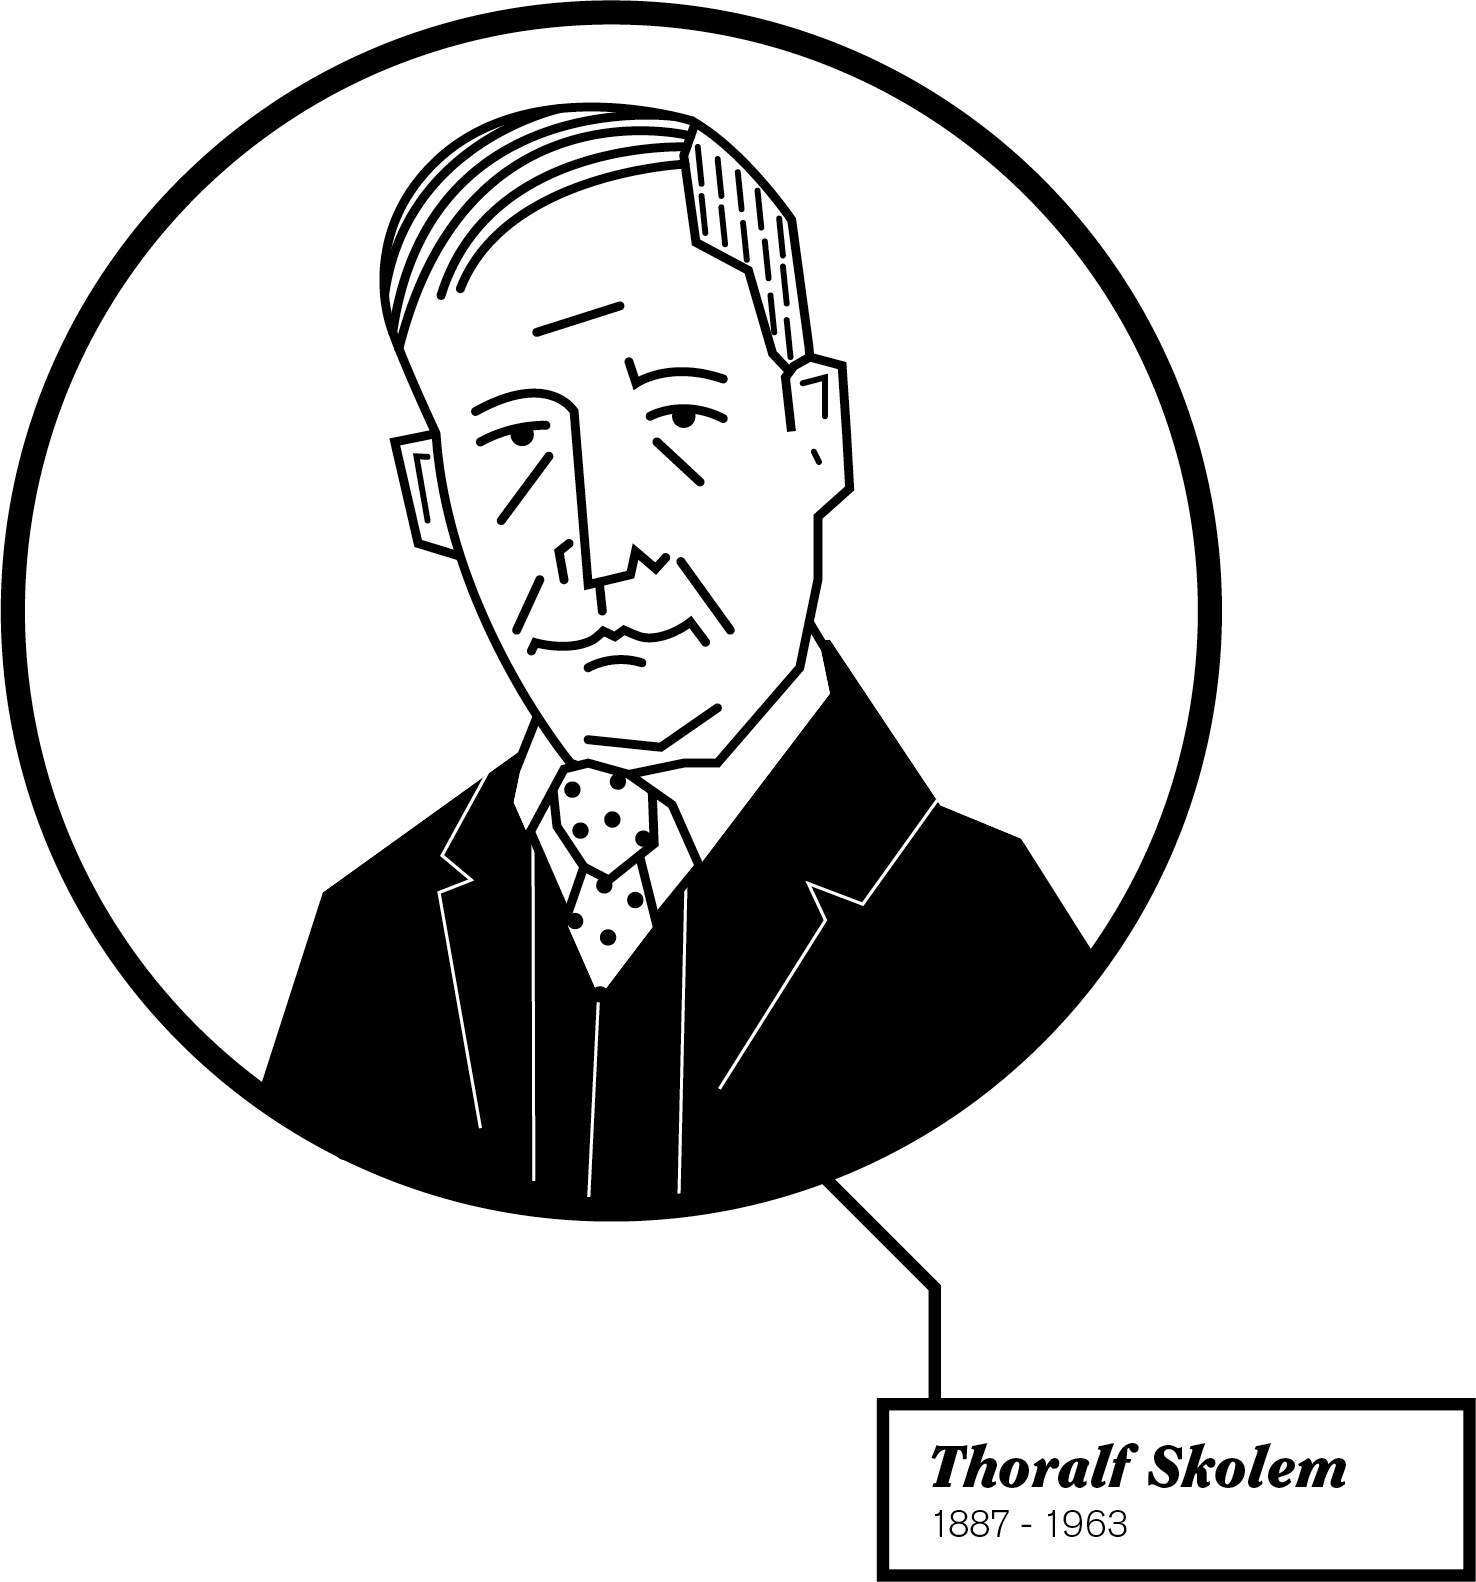
\includegraphics[width=\textwidth]{illustrations/SkolemChapter}
\vfill

\chapter{Prefácio}

Este livro é uma introdução à metalógica, voltada especialmente a
estudantes de ciência da computação e de filosofia. «Metalógica» é
assim chamada porque é a disciplina que estuda a própria lógica. A
lógica propriamente dita trata dos cânones de inferência válida, e sua
versão simbólica ou formal apresenta esses cânones usando linguagens
formais, como as da lógica proposicional e da lógica de primeira
ordem. A metalógica investiga as propriedades dessas linguagens e dos
cânones de inferência correta que as utilizam. Ela estuda tópicos como
o de dar significado preciso às expressões dessas linguagens formais,
como justificar os cânones de inferência válida, quais são as
propriedades de vários sistemas de !!{derivation}, incluindo suas
propriedades computacionais. Essas questões são importantes e
interessantes por si mesmas, porque as linguagens e os sistemas de
!!{derivation} investigados são aplicados em muitas áreas
diferentes---em matemática, filosofia, ciência da computação e
linguística, especialmente---, mas também servem como exemplos de como
estudar sistemas formais em geral. As linguagens lógicas que estudamos
aqui não são as únicas de interesse. Por exemplo, linguistas e
filósofos se interessam por linguagens muito mais complicadas do que as
da lógica proposicional e da lógica de primeira ordem, e cientistas da
computação se interessam por \emph{outros tipos} de linguagens, como
linguagens de programação. E os métodos que discutimos---como dar
semântica a linguagens formais, como provar resultados sobre linguagens
formais, como investigar as propriedades de linguagens formais---também
são aplicáveis nesses casos.

Como qualquer disciplina, a metalógica tem um conjunto de resultados ou
fatos e um repertório de métodos e técnicas, e este texto cobre ambos.
Muitos estudantes não precisarão conhecer todos os resultados que
discutimos fora deste curso, mas precisarão e usarão os métodos que
empregamos para estabelecê-los. O teorema de Löwenheim-Skolem, por
exemplo, não aparece com frequência em ciência da computação, mas os
métodos que usamos para prová-lo sim. Por outro lado, muitos dos
resultados que discutimos têm relevância para certos debates, digamos,
na filosofia da ciência e na metafísica. Estudantes de filosofia podem
não precisar ser capazes de provar esses resultados fora deste curso,
mas precisam entender quais são os resultados---e você só
\emph{entende} de fato esses resultados se refletiu sobre as
definições e provas necessárias para estabelecê-los. Essas são, em
parte, as razões pelas quais os resultados e os métodos cobertos neste
texto são estudo recomendado---em alguns casos até obrigatório---para
estudantes de ciência da computação e de filosofia.

O material está dividido em três partes. A \olref[sfr][][]{part} trata
da teoria dos conjuntos. Lógica e metalógica estão historicamente muito
ligadas ao que se chama «fundamentos da matemática». Os fundamentos
matemáticos tratam de como, em última instância, objetos matemáticos
como inteiros, racionais e reais, funções, espaços etc. devem ser
entendidos. A teoria dos conjuntos fornece uma resposta (há outras), e
por isso teoria dos conjuntos e lógica há muito são estudadas em
paralelo. Conjuntos, relações e funções também são onipresentes em
qualquer investigação formal, não só em matemática, mas também em
ciência da computação e em alguns cantos mais técnicos da filosofia.
Certamente, para formular e provar resultados sobre semântica e teoria
da prova da lógica e sobre os fundamentos da computabilidade, é
essencial dispor de uma terminologia para isso. Por exemplo, falaremos
de conjuntos de expressões, relações de consequência e de
demonstrabilidade, interpretações de símbolos de predicado (que se
revelam relações), funções computáveis e várias relações e construções
que as envolvem. Será bom ter símbolos abreviados para isso e refletir
sobre as propriedades gerais de conjuntos, relações e funções. Se você
não está acostumado a pensar matematicamente e a formular provas
matemáticas, pense na primeira parte sobre teoria dos conjuntos como
um campo de treino: todas as definições básicas serão dadas, e
apresentaremos provas cada vez mais complicadas usando-as. Note que
entender essas provas---e ser capaz de encontrá-las e formulá-las
você mesmo---é talvez mais importante do que entender os resultados,
especialmente na primeira parte. Se o pensamento matemático é novo para
você, é importante que você reflita sobre os exemplos e problemas.

Na primeira parte estabeleceremos um resultado importante, no entanto.
Esse resultado---o teorema de Cantor---depende de um dos exemplos mais
marcantes de análise conceitual que se encontra nas ciências, a saber,
a análise do infinito por Cantor. O infinito intrigou matemáticos e
filósofos por séculos. Até Cantor, ninguém sabia como pensar
adequadamente sobre ele. Muitas pessoas chegaram a considerar um erro
pensar sobre o infinito e acreditavam que a noção de coleção infinita
em si era incoerente. Cantor transformou o infinito em um assunto com
o qual podemos trabalhar de forma coerente e desenvolveu toda uma
teoria de coleções infinitas---e números infinitos com os quais
podemos medir os tamanhos de coleções infinitas. Ele mostrou que há
diferentes níveis de infinito. Essa teoria de números «transfinitos» é
bela e intricada, e não nos aprofundaremos muito nela; mas seremos
capazes de mostrar que há diferentes níveis de infinito,
especificamente, que há níveis «contáveis» e «incontáveis» de
infinito. Esse resultado tem aplicações importantes, mas também é
realmente o tipo de resultado que qualquer matemático, cientista da
computação e filósofo que se preze deveria conhecer.

Na \olref[fol][][]{part}, passamos à lógica de primeira ordem.
Definiremos a linguagem da lógica de primeira ordem e sua semântica,
isto é, o que são estruturas de primeira ordem e quando uma sentença
da lógica de primeira ordem é verdadeira numa estrutura. Isso nos
permitirá fazer duas coisas importantes: (1)~podemos definir, com
precisão matemática, quando uma sentença é consequência lógica de
outra; (2)~também podemos considerar como as relações que compõem uma
estrutura de primeira ordem são descritas---caracterizadas---pelas
sentenças que são verdadeiras nelas. Isso nos leva, em particular, a
uma discussão do método axiomático, no qual sentenças de linguagens de
primeira ordem são usadas para caracterizar certos tipos de estruturas.
A teoria da prova nos ocupará em seguida, e consideraremos a versão
original do cálculo de sequentes e da dedução natural definidas na
década de 1930 por Gerhard Gentzen. (Seu professor pode optar por
cobrir apenas um deles; então qualquer referência a
«!!{derivation}s» e «!!{derivability}» significará o sistema que ele
escolheu.) A noção semântica de consequência e a noção sintática de
!!{derivability} nos dão duas maneiras completamente diferentes de
tornar precisa a ideia de que uma sentença pode seguir de outras. Os
teoremas de correção e completude ligam essas duas caracterizações.
Em particular, provaremos o teorema da completude de Gödel, que
afirma que sempre que uma sentença é consequência semântica de outras,
ela também é !!{derivable} a partir delas. Uma formulação equivalente
é: se uma coleção de sentenças é consistente---no sentido de que nada
contraditório pode ser provado a partir delas---, então existe uma
estrutura que torna todas elas verdadeiras.

A segunda formulação do teorema da completude é talvez a mais
surpreendente. Por volta da época em que Gödel provou esse resultado
(em 1929), o matemático alemão David Hilbert defendia famosamente a
visão de que consistência (isto é, ausência de contradição) é tudo o
que a existência matemática exige. Em outras palavras, sempre que um
matemático pode descrever coerentemente uma estrutura ou classe de
estruturas, ele deveria ter o direito de acreditar na existência
dessas estruturas. Na época, muitos achavam essa ideia absurda: só
porque você pode descrever uma estrutura sem se contradizer, certamente
não se segue que tal estrutura realmente existe. Mas é exatamente isso
que o teorema da completude de Gödel diz. Além desse aspecto
paradoxal---e certamente intrigante do ponto de vista filosófico---, o
teorema da completude também tem duas aplicações importantes que nos
permitem provar outros resultados sobre a existência de estruturas que
tornam certas sentenças verdadeiras. São os teoremas da compacidade e
de Löwenheim-Skolem.

Na \olref[tur][][]{part}, conectamos lógica e computabilidade. De
novo, há uma conexão histórica: David Hilbert havia colocado como
problema fundamental da lógica encontrar um método mecânico que
decidisse, para uma dada sentença da lógica, se ela tem uma prova. Tal
método existe, é claro, para a lógica proposicional: basta verificar
todas as tabelas-verdade, e como há apenas um número finito delas, o
método eventualmente produz uma resposta correta. Um método tão direto
não é possível para a lógica de primeira ordem, já que o número de
estruturas possíveis é infinito (e as próprias estruturas podem ser
infinitas). Lógicos trabalharam por anos para encontrar métodos mais
engenhosos. Alonzo Church e Alan Turing acabaram estabelecendo que não
existe tal método. Para fazer isso, foi necessário primeiro fornecer uma
definição precisa do que é, em geral, um método mecânico. Se um
procedimento de decisão tivesse sido proposto, presumivelmente ele
teria sido reconhecido como um método efetivo. Para provar que nenhum
método efetivo existe, é preciso definir «método efetivo» primeiro e
dar uma prova de impossibilidade com base nessa definição. Foi isso
que Turing fez: ele propôs a ideia de uma máquina de
Turing\footnote{Turing, é claro, não a chamou assim.} como modelo
matemático do que um procedimento mecânico pode, em princípio, fazer.
Esse é outro exemplo de \emph{análise conceitual} de um conceito
informal usando maquinaria matemática; e talvez seja de importância
comparável para a ciência da computação à análise do infinito por
Cantor para a matemática. Nossa última grande empreitada será a prova
de dois teoremas de impossibilidade: mostraremos que o chamado
«problema da parada» não pode ser resolvido por máquinas de Turing e,
por fim, que o «problema da decisão» de Hilbert (para a lógica)
também não pode.

Este texto é matemático, no sentido de que discutimos definições
matemáticas e provamos nossos resultados matematicamente. Mas não é
matemático no sentido de que você precise de amplo conhecimento prévio
de matemática. Nada neste texto exige conhecimento de álgebra,
trigonometria ou cálculo. Fizemos um esforço especial para também não
exigir familiaridade com o modo de trabalho da matemática: de fato,
parte do objetivo é \emph{desenvolver} os tipos de raciocínio e
habilidades de prova necessários para entender e provar nossos
resultados. A organização do texto segue a convenção matemática, por um
motivo: essas convenções foram desenvolvidas porque clareza e precisão
são especialmente importantes, e assim, por exemplo, é crucial saber
quando algo é afirmado como conclusão de um argumento, é oferecido
como razão para outra coisa ou pretende introduzir novo vocabulário.
Por isso seguimos a convenção matemática e rotulamos passagens como
«definições» se servem para introduzir nova terminologia ou símbolos; e
como «teoremas», «proposições», «lemas» ou «corolários» quando
registramos um resultado ou achado. Fora essas convenções, usaremos os
métodos de prova lógica que talvez já sejam familiares de um primeiro
curso de lógica, e também faremos amplo uso do método de
\emph{indução} para provar resultados. Dois capítulos do apêndice são
dedicados a esses métodos de prova.

\paragraph{Notas para instrutores} O material deste livro é adequado
para um segundo curso semestral de lógica formal. Eu o cubro em 12
semanas em Lógica~II na University of Calgary, embora não cubra tudo
com o mesmo nível de detalhe que há neste livro. Por exemplo,
normalmente trato apenas de dedução natural e deixo de fora provas
detalhadas de completude para identidade. Os estudantes já cursaram
Lógica~I, normalmente a partir de
\emph{\href{https://forallx.openlogicproject.org}{forall x: Calgary}},
que usa as mesmas regras de dedução natural, exceto no formato Fitch.

A versão mais recente deste livro está disponível em PDF em
\href{https://slc.openlogicproject.org}{slc.openlogicproject.org}, mas
muda com frequência. A licença CC BY lhe dá o direito de baixar e
distribuir o livro você mesmo. Para garantir que todos os seus
estudantes tenham a mesma versão do livro durante o semestre em que o
usam, você deve fazê-lo: envie o PDF que decidir usar para o seu LMS
em vez de apenas dar aos estudantes o link. Você também pode mandar
imprimir os PDFs na livraria da universidade, mas algumas livrarias
poderão comprar e estocar os livros de capa mole disponíveis na Amazon.

A sintaxe, a semântica e os sistemas de prova da lógica de primeira
ordem são apoiados pelo aplicativo gratuito e online de ensino de
lógica \emph{Carnap}, de Graham Leach-Krouse
(\href{https://carnap.io}{carnap.io}). Isso permite envio e correção
automática de exercícios como !!{derivation}s de dedução natural e de
cálculo de sequentes, fornecimento de estruturas para teorias simples
e exercícios de simbolização. Há também um simulador de máquinas de
Turing em
\href{https://turing.openlogicproject.org}{turing.openlogicproject.org}
que pode ser usado para ilustrar o material da \olref[tur][][]{part}.
Os exemplos lá estão disponíveis pré-carregados no simulador.


\cleartoverso 


\thispagestyle{empty}
\ \vfill
\noindent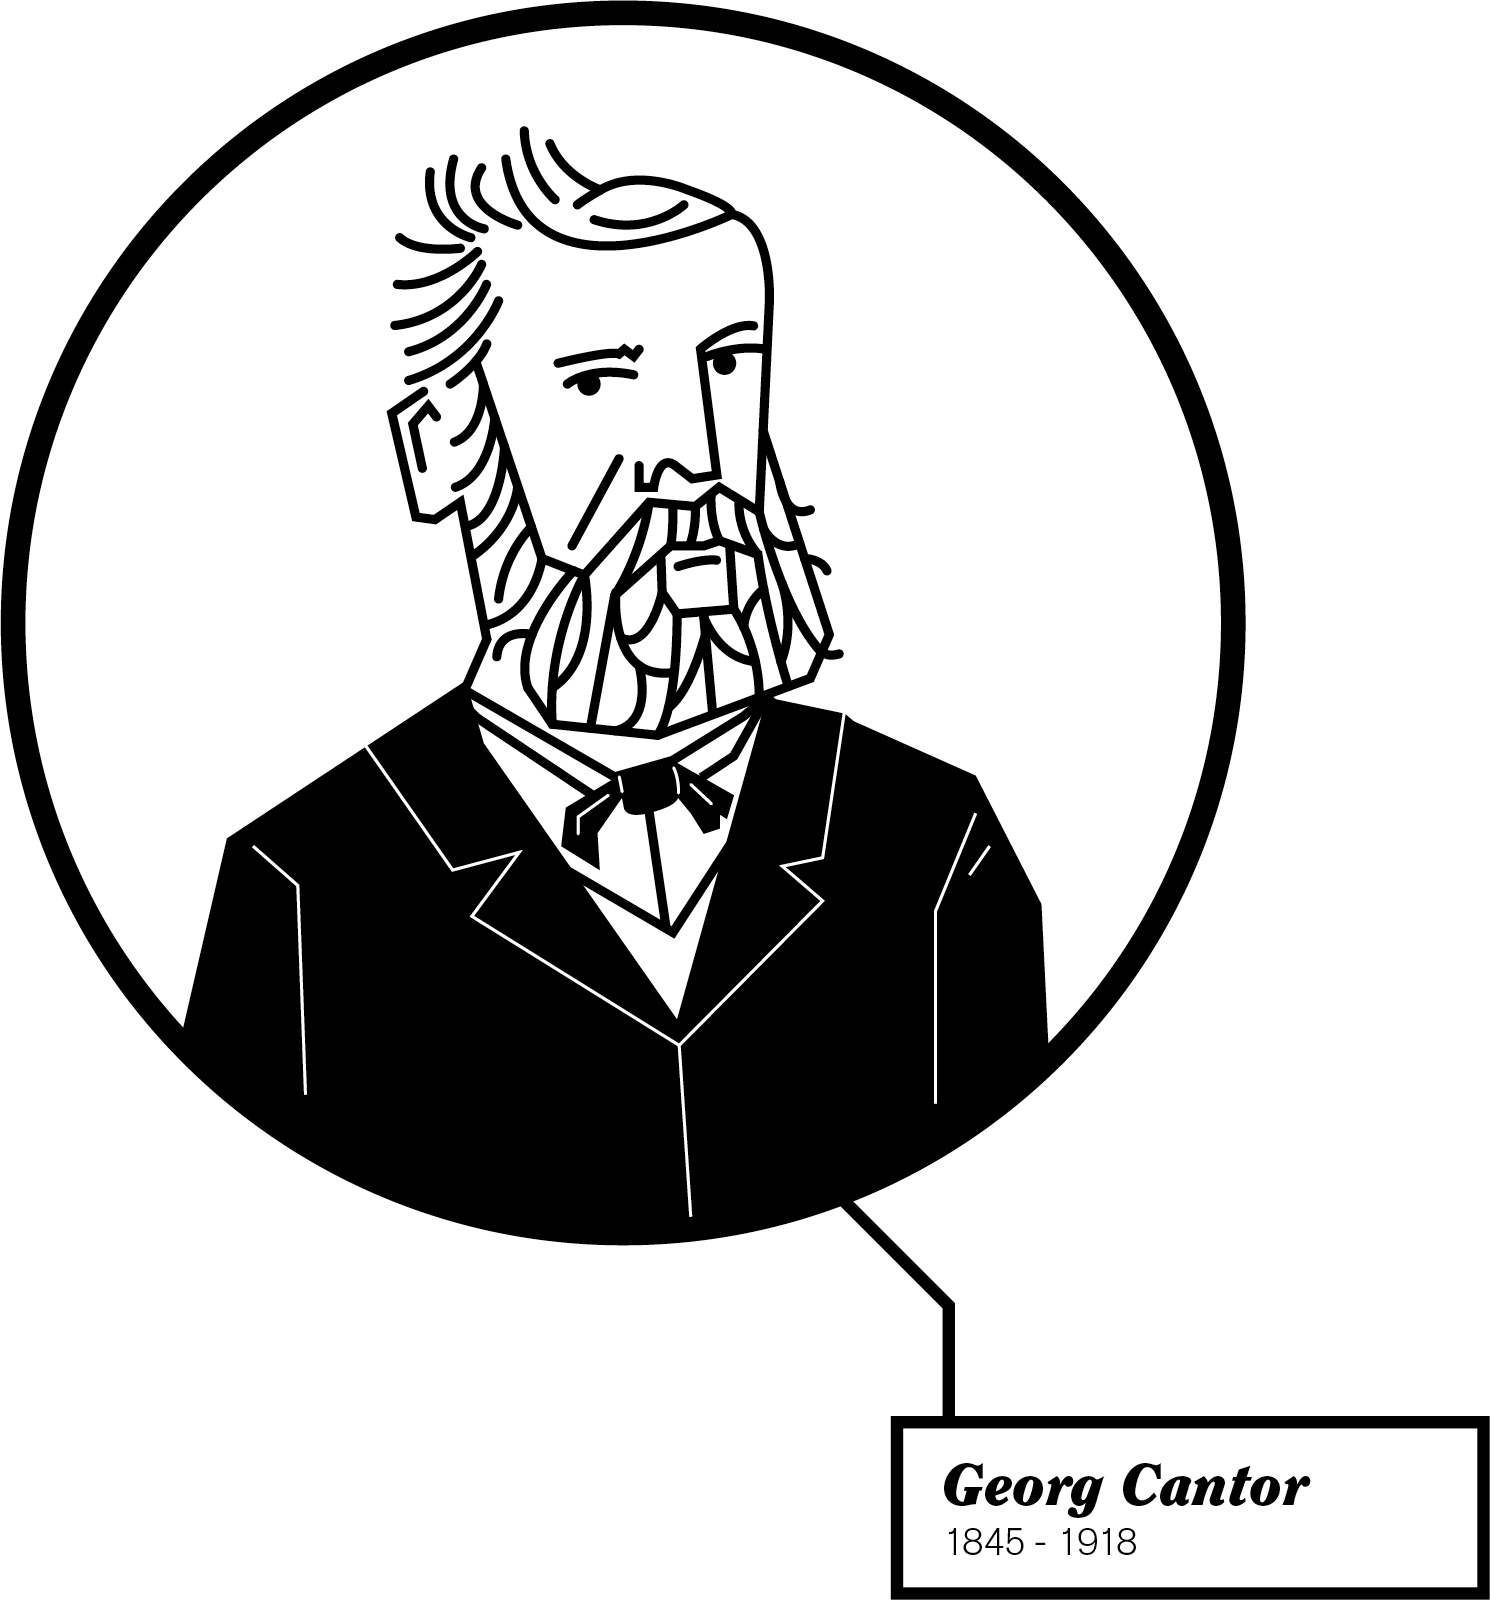
\includegraphics[width=\textwidth]{illustrations/CantorChapter}
\vfill

\mainmatter

\olimport*[sets-functions-relations]{sets-functions-relations}

\cleartoverso
\ifodd\value{page}\stepcounter{page}\fi
\thispagestyle{empty}
\ \vfill
\noindent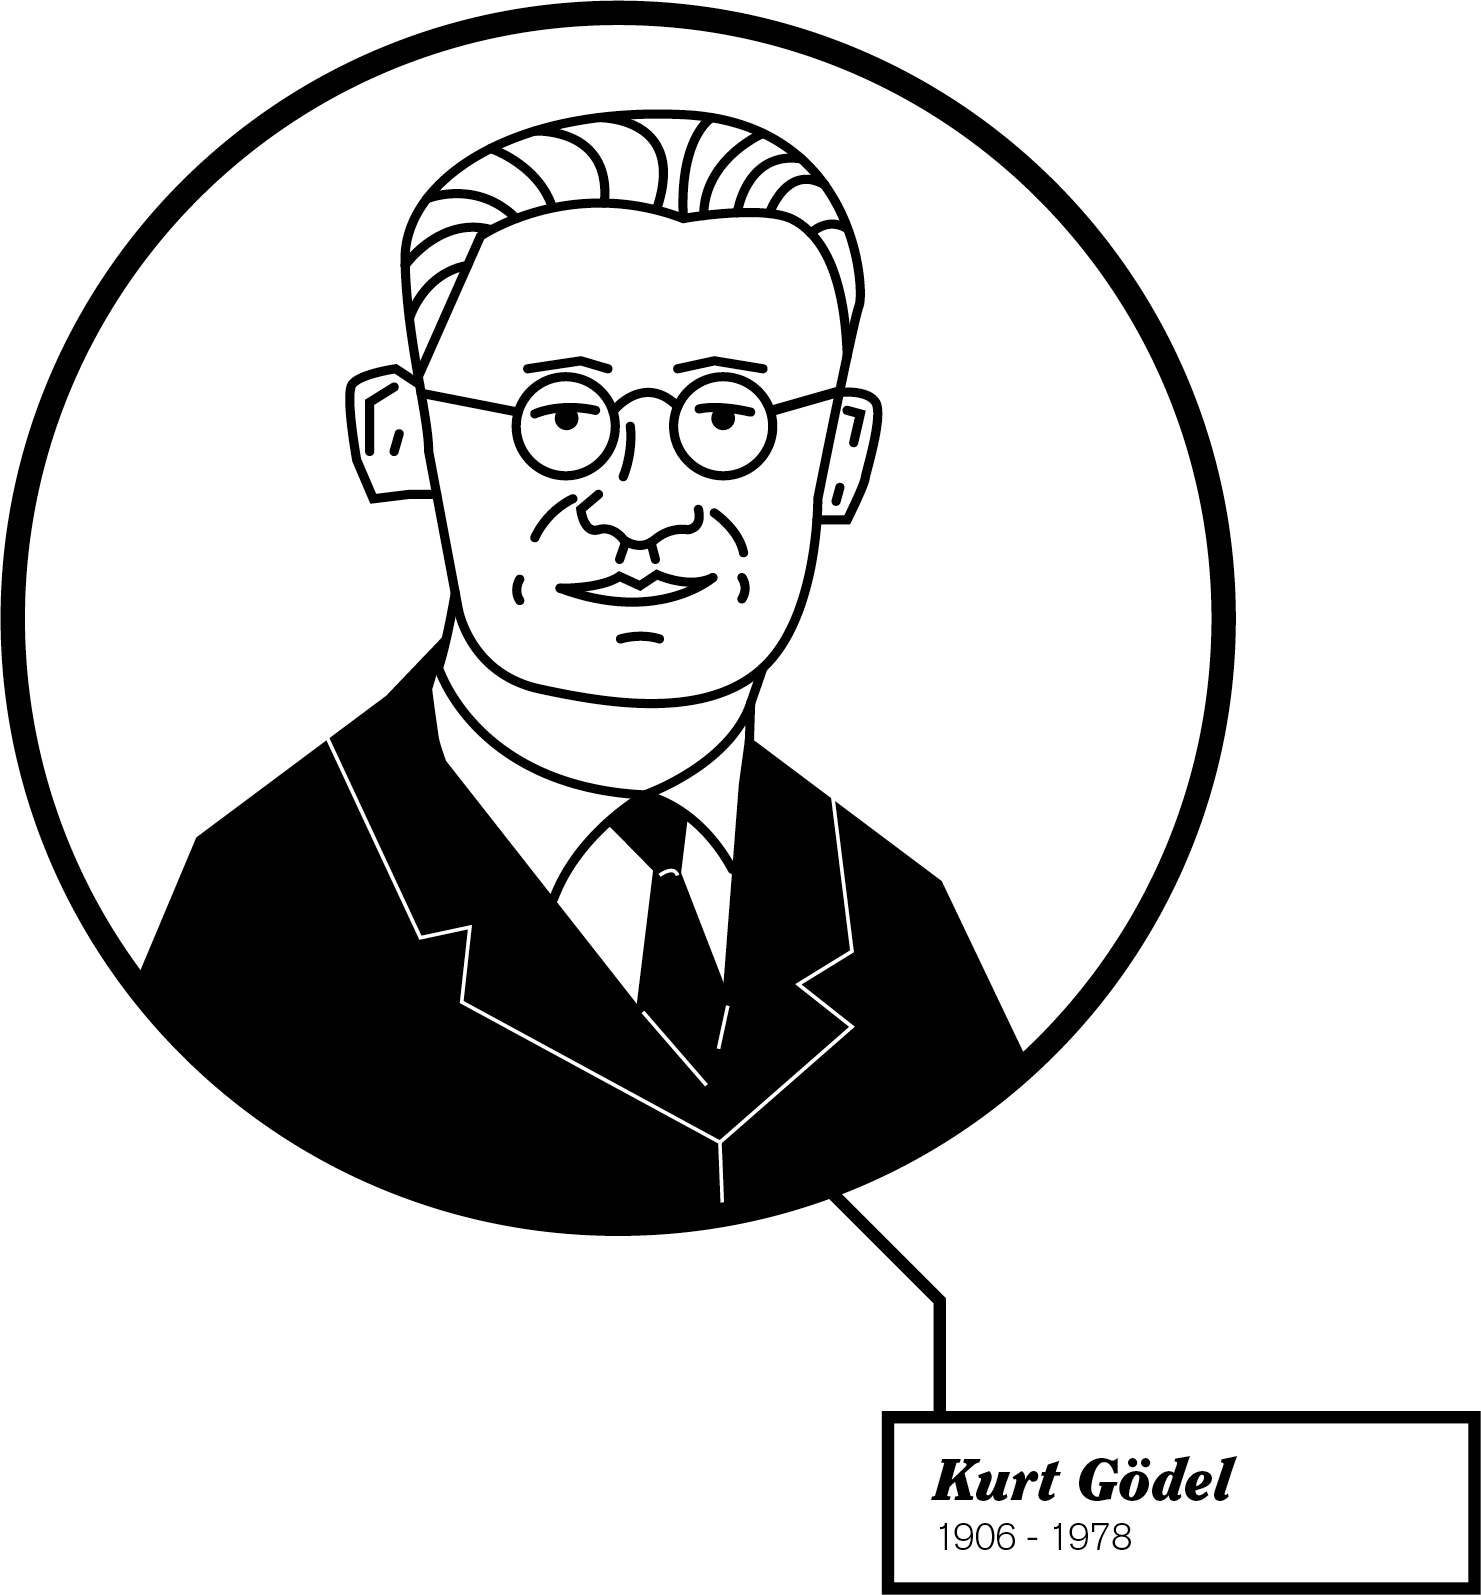
\includegraphics[width=\textwidth]{illustrations/GodelChapter}
\vfill

\olimport*[first-order-logic]{first-order-logic}

\cleartoverso
\ifodd\value{page}\stepcounter{page}\fi
\thispagestyle{empty}
\ \vfill
\noindent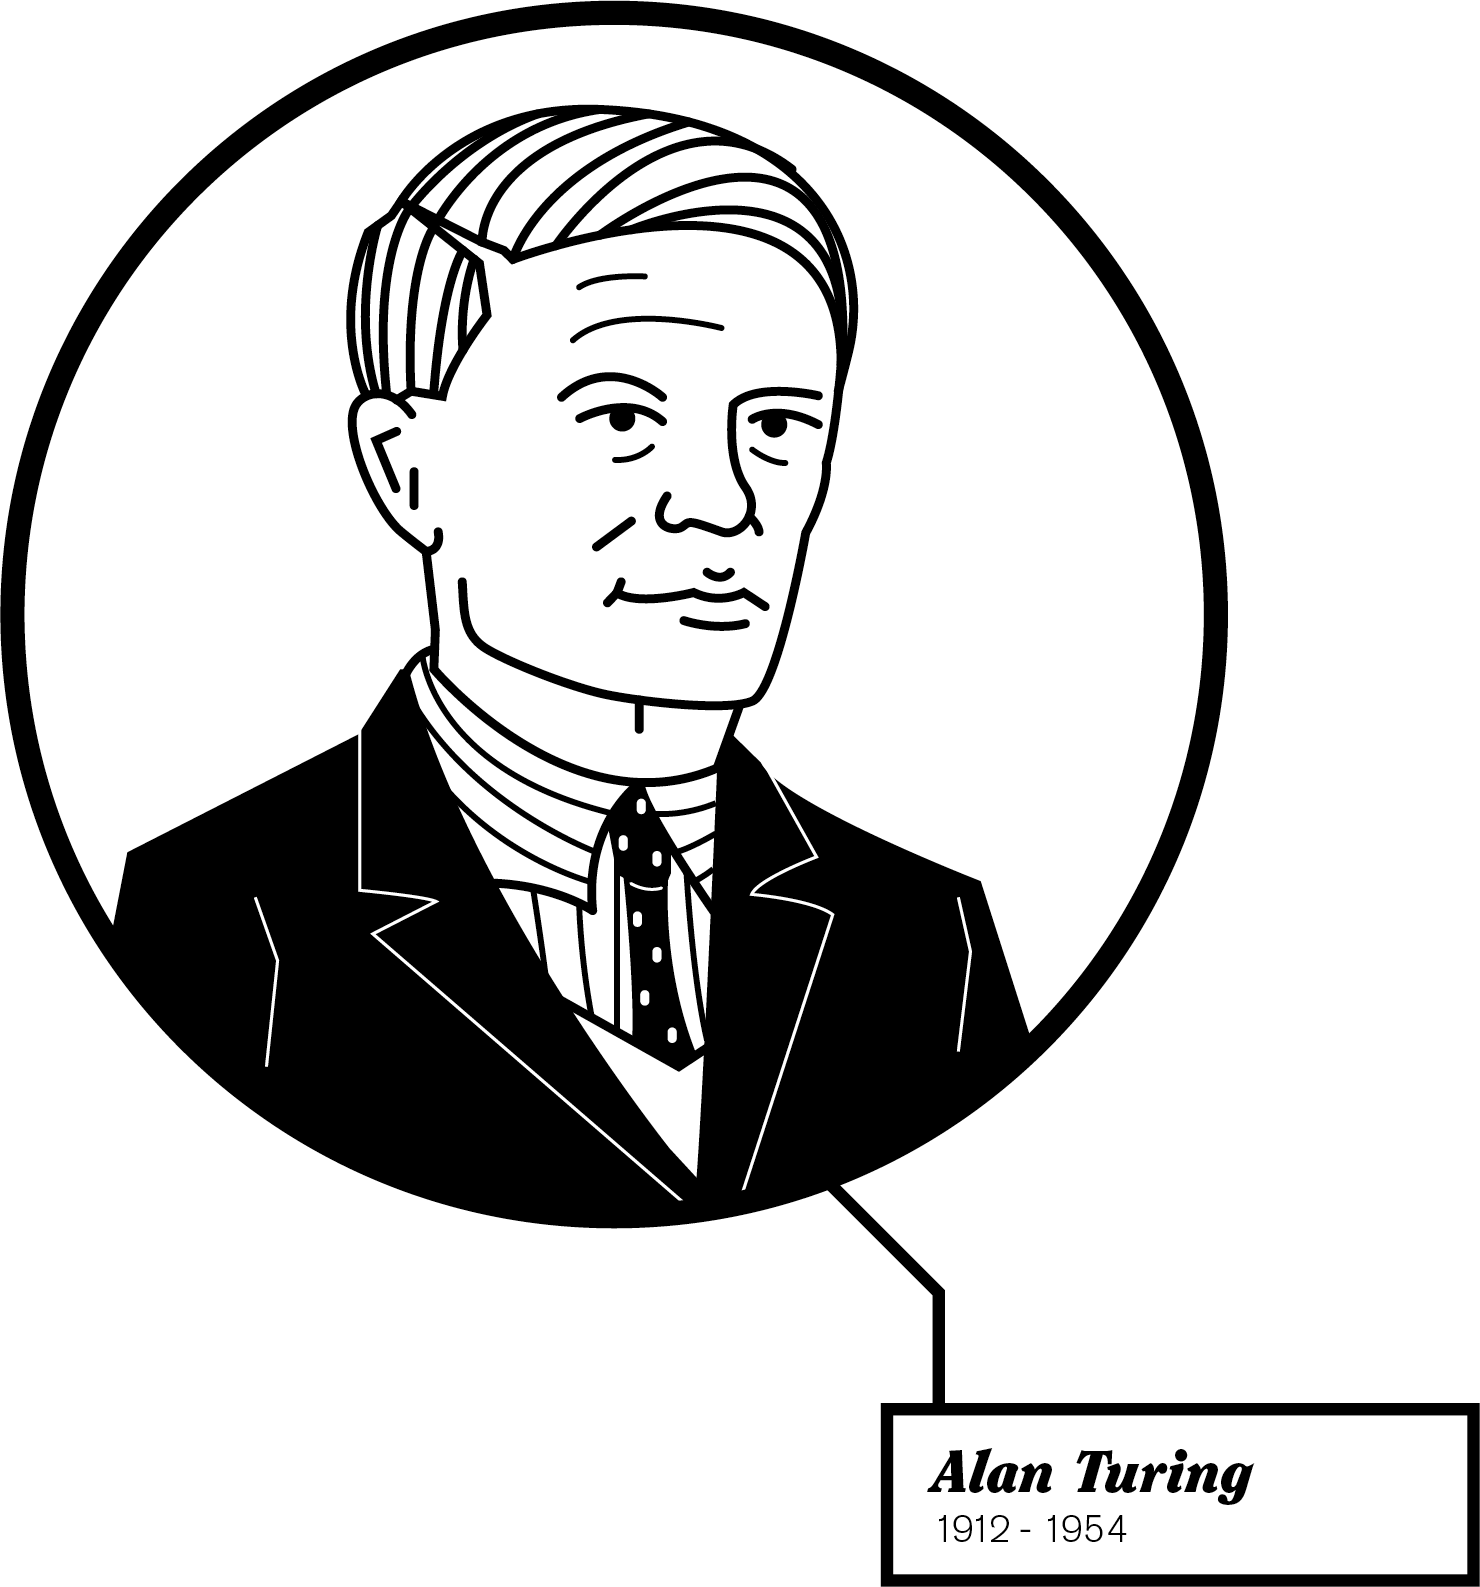
\includegraphics[width=\textwidth]{illustrations/TuringChapter}
\vfill

\olimport*[turing-machines]{turing-machines}

% appendices

\cleartoverso
\ifodd\value{page}\stepcounter{page}\fi
\thispagestyle{empty}
\ \vfill
\noindent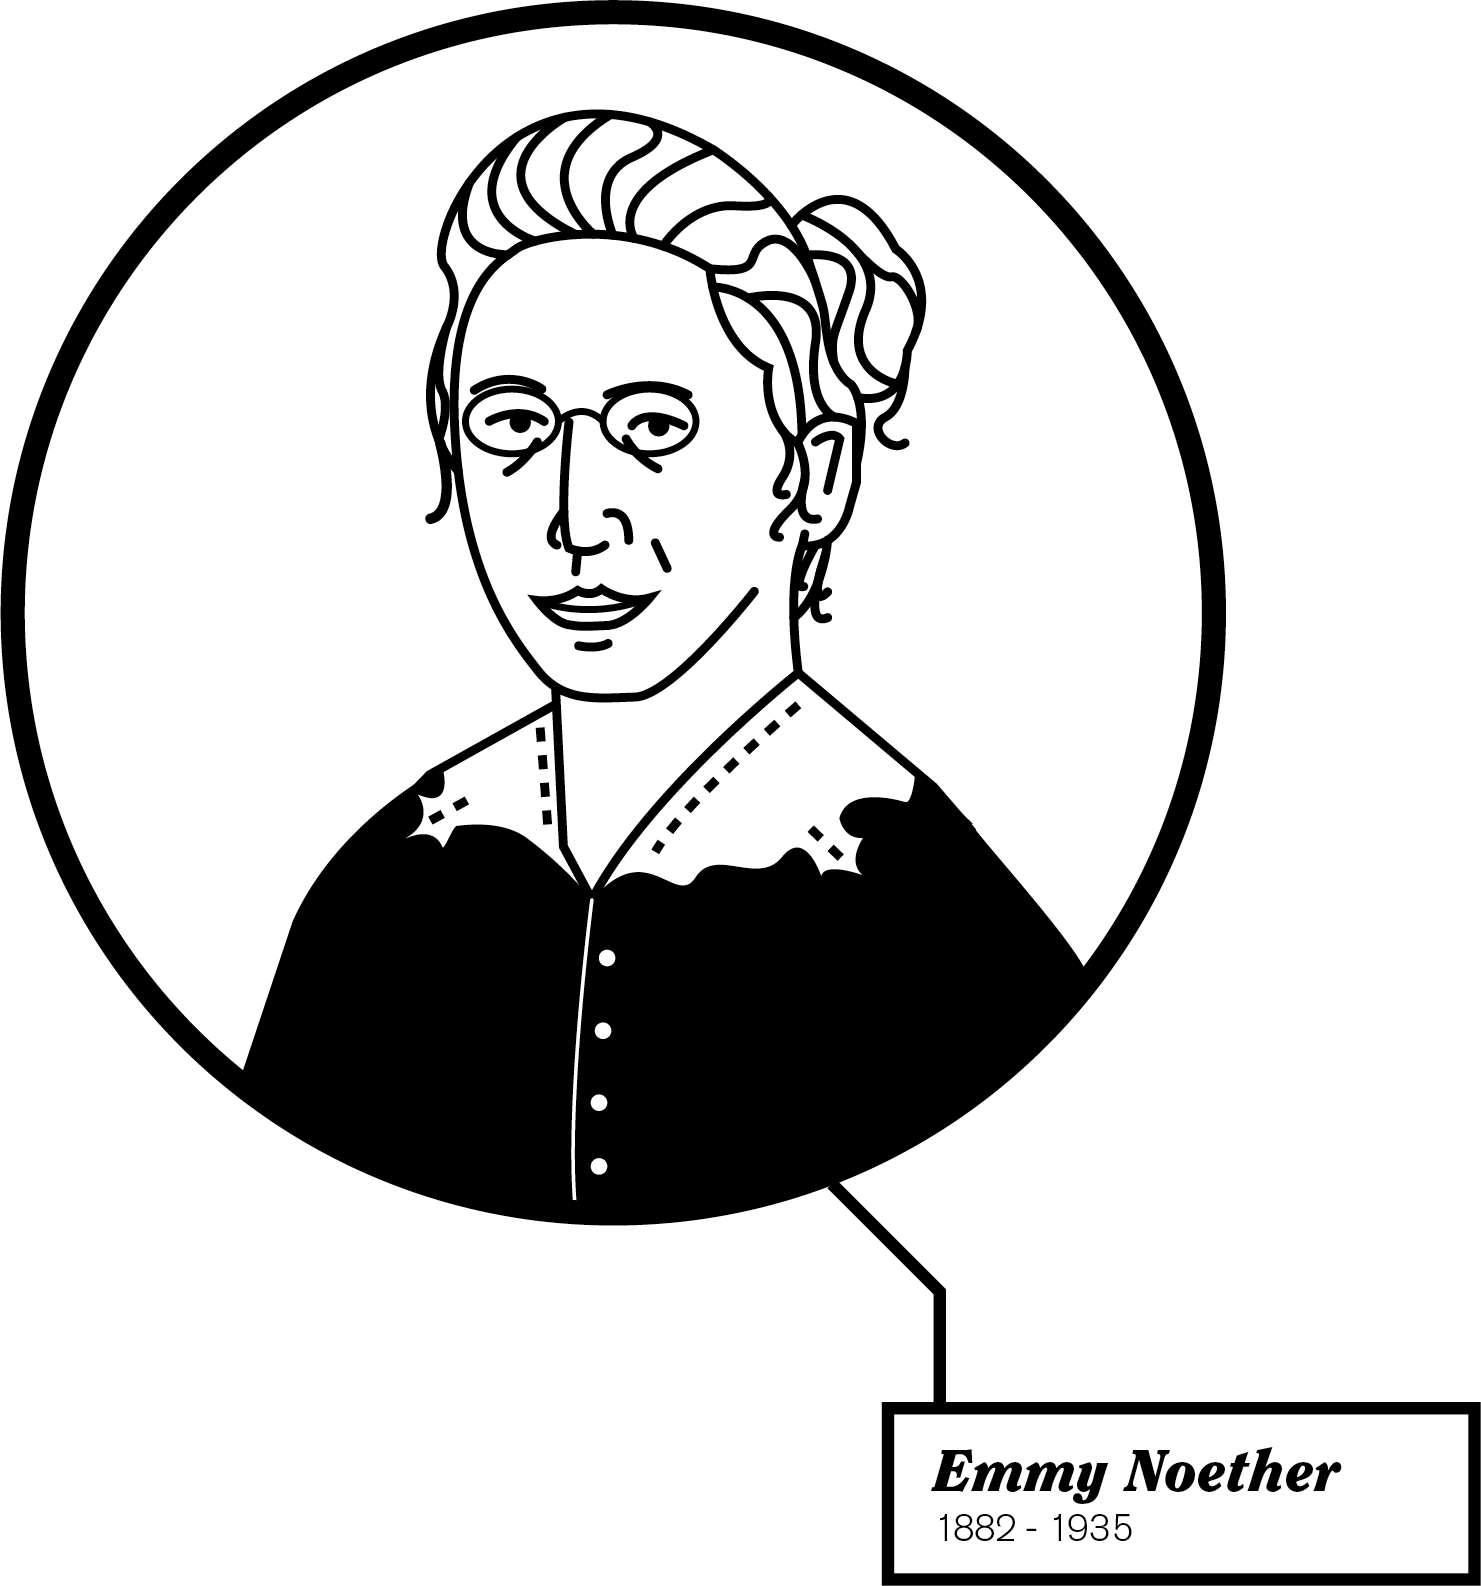
\includegraphics[width=\textwidth]{illustrations/NoetherChapter}
\vfill

\appendix

\olimport*[methods/proofs]{proofs}

\olimport*[methods/induction]{induction}

\stopproblems
\def\ifproblems#1{}

\def\figurename{Fig.}
\setlength{\olphotowidth}{.45\textwidth}

\chapter{Biografias}

\olimport*[history/biographies]{georg-cantor}

\olimport*[history/biographies]{alonzo-church}

\olimport*[history/biographies]{gerhard-gentzen}

\olimport*[history/biographies]{kurt-goedel}

\olimport*[history/biographies]{emmy-noether}

\olimport*[history/biographies]{bertrand-russell}

\olimport*[history/biographies]{alfred-tarski}

\olimport*[history/biographies]{alan-turing}

\olimport*[history/biographies]{ernst-zermelo}

\olimport*[reference/greek-alphabet]{greek-alphabet}

%\backmatter

\glsaddall
\printglossaries

\clearpage
\photocredits

\bibliographystyle{\olpath/locale/pt/bib/natbib-oup-pt}
\bibliography{\olpath/bib/open-logic.bib}

\olimport*[]{open-logic-about}


\end{document}